\documentclass{article}
\usepackage{graphicx}  
\usepackage{listings}
\usepackage{subcaption}
\usepackage{caption}

\lstset{
	basicstyle=\ttfamily\small,  % Police machine à écrire, taille réduite
	numbers=left,                % Numérotation des lignes à gauche
	numberstyle=\tiny,           % Taille réduite pour les numéros de ligne
	stepnumber=1,                % Numérotation à chaque ligne
	frame=single,                % Encadrer le code
	breaklines=true,             % Autoriser les retours à la ligne
	showstringspaces=false,      % Ne pas afficher les espaces dans les chaînes
	tabsize=4,                   % Largeur des tabulations
	captionpos=b,                % Position de la légende (en bas)
}

\title{Premières simulations DUST}
\author{Alexandre Laleu}
\date{\today}

\begin{document}
	
	\maketitle
	\section{Présentation des données}
	Toutes les données utilisées ici s'appuient sur les résultats des codes d'optimisation de Boqiao du challenge ONERA 2024. \\Ces données proviennent d'algorithmes cherchant à optimiser le bruit, la portance et la puissance consommée en ajustant deux valeurs : la cordre (chord) et le vrillage (twist) en construisant un front de pareto.\\
	Les résultats sont les suivants : 
	\begin{figure}[h]
		\centering
		\includegraphics[width=1\textwidth]{données_Boqiao.jpg}
		\caption{Valeurs de corde et de vrillages optimisées}
		\label{fig:image}
	\end{figure}
	\section{Objectif des simulations}
	Nous allons ici utiliser la simulation pour trouver les RPM optimum qui nous permettent d'atteindre la portance cible de 4,5N.\\
	Pour ce faire, on lance les simulations pour trois valeurs de RPM distincts pour relever la portance produite à ces RPM et on calcule le polynôme de degré deux passant par ces points sur python.\\
	Par manque de temps (certaines simulations pour les pales à 14 segments prenaient 45 min de calcul à mon ordinateur), je me suis limité aux traitement des tableaux 1 et 3.
	
	
	\section{Brève explication des codes}
	Les codes calculent la portance et le moment via la méthode des \verb !sectional loads!. C'est à dire que le calcul des différentes grandeurs est effectué indépendamment sur chaque région de la pâle définie dans le fichier \verb!ll_wing.in!.\\ \\
	Chaque pale de l'hélice a une envergure de $\frac{23.9}{2}=11.95$cm auxquels il convient de retirer le rayon du moyeu de l'hélice, imposé à 4mm par l'ONERA (confirmez moi ceux du banc d'essai svp). \\La simulation prend en compte le moyeu avec la définition de \\ \verb! starting_point = (/0.0, 0.004, 0.0/)! dans le fichier \verb!ll_wing.in!. \\\\
	L'envergure (span) des régions associées au tableau 1 (8 régions) est donc de $span = 1.44$cm.\\ \\
	De même, celle du tableau 3 (13 régions) est $span = 0.888$cm.\\ \\
	Pour chaque simulation, il faut aussi veiller à changer \verb !u_ref!$ = r_{pale}$\verb!*RPM! dans le fichier \verb!dust.in!.\\ \\
	La vitesse de rotation est quant à elle définie en rad/s dans le fichier \verb!References.in! avec la variable \verb!rot rate!.\\ \\
	 Les simulations tournent sur 6 révolutions de la pâle pendant son régime stationnaire : \verb !tstart = 0.0, tend =0.072! dans \verb!dust.in! pour définir les 6 révolutions et \verb!start_res = 301, end_res = 361! dans \verb!dust_post! pour la période en régime stationnaire (ces dernières données sont issus d'anciennes simulations sur lesquelles j'ai repéré l'ordre de grandeur des temps du régime stationnaire). \\ \\
	 \verb!Casalino_plot_Fz/Mo.py! du dossier \verb!python!. \\ \\ 
	Le profil de chaque région est en NACA4412. \\ \\
	Tous les résultats sont traités par python qui va sommer les portances de toutes les régions avec les fichiers. On retiendra la moyenne temporelle de la portance dans l'interpolation avec le polynôme (cf  dossier \verb!optimisation_RPM!).\\ \\
	Les valeurs de $twist$ et $chord$ proviennent des tableaux de Boqiao présentés dans le premier paragraphe. \\ \\
	Vous trouverez en page suivante un exemple de \verb!ll_wing.in! :  \clearpage
	\begin{lstlisting}
		mesh_file_type = parametric
		el_type = l
		starting_point = (/0.0, 0.004, 0.0/)
		reference_chord_fraction = 0.0
		
		!Section 1
		chord = 0.025
		twist = 45
		airfoil_table = ./airfoil_table/naca4412.c81
		
		!Region 1
		span = 0.0144375
		sweep = 0
		dihed = 0
		nelem_span = 7
		type_span = uniform
		
		!Section 2
		chord = 0.0334
		twist = 34
		airfoil_table = ./airfoil_table/naca4412.c81
		
		!Region 2
		span = 0.0144375
		sweep = 0
		dihed = 0
		nelem_span = 7
		type_span = uniform
		
		!Section 3
		chord = 0.0341
		twist = 29
		airfoil_table = ./airfoil_table/naca4412.c81
		
		!Region 3
		span = 0.0144375
		sweep = 0
		dihed = 0
		nelem_span = 7
		type_span = uniform
		
		!Section 4
		chord = 0.0341
		twist = 23
		airfoil_table = ./airfoil_table/naca4412.c81
		
		etc ...
	\end{lstlisting}
	\section{Résultats des simulations}
% Première partie de la figure
\begin{figure}[h]
	\centering
	
	% Première ligne : 2 pales, 3000 RPM
	\begin{subfigure}{0.45\textwidth}
		\includegraphics[width=\linewidth]{C:/Users/laleu/OneDrive/Documents/2A/DUST-CFD/Casalino/Hover_LL_3_donnees_Boqiao/Hover_LL_3_tableau1/python/resultats_3000RPM_Fz.PNG}
		\caption{Portance - 2 pales à 3000RPM}
	\end{subfigure}
	\hfill
	\begin{subfigure}{0.45\textwidth}
		\includegraphics[width=\linewidth]{C:/Users/laleu/OneDrive/Documents/2A/DUST-CFD/Casalino/Hover_LL_3_donnees_Boqiao/Hover_LL_3_tableau1/python/resultats_3000RPM_Mo.PNG}
		\caption{Moment - 2 pales à 3000RPM}
	\end{subfigure}
	
	% Deuxième ligne : 2 pales, 5000 RPM
	\begin{subfigure}{0.45\textwidth}
		\includegraphics[width=\linewidth]{C:/Users/laleu/OneDrive/Documents/2A/DUST-CFD/Casalino/Hover_LL_3_donnees_Boqiao/Hover_LL_3_tableau1/python/resultats_5000RPM_Fz.PNG}
		\caption{Portance - 2 pales à 5000RPM}
	\end{subfigure}
	\hfill
	\begin{subfigure}{0.45\textwidth}
		\includegraphics[width=\linewidth]{C:/Users/laleu/OneDrive/Documents/2A/DUST-CFD/Casalino/Hover_LL_3_donnees_Boqiao/Hover_LL_3_tableau1/python/resultats_5000RPM_Mo.PNG}
		\caption{Moment - 2 pales à 5000RPM}
	\end{subfigure}
	
	% Troisième ligne : 2 pales, 8000 RPM
	\begin{subfigure}{0.45\textwidth}
		\includegraphics[width=\linewidth]{C:/Users/laleu/OneDrive/Documents/2A/DUST-CFD/Casalino/Hover_LL_3_donnees_Boqiao/Hover_LL_3_tableau1/python/resultats_8000RPM_Fz.PNG}
		\caption{Portance - 2 pales à 8000RPM}
	\end{subfigure}
	\hfill
	\begin{subfigure}{0.45\textwidth}
		\includegraphics[width=\linewidth]{C:/Users/laleu/OneDrive/Documents/2A/DUST-CFD/Casalino/Hover_LL_3_donnees_Boqiao/Hover_LL_3_tableau1/python/resultats_8000RPM_Mo.PNG}
		\caption{Moment - 2 pales à 8000RPM}
	\end{subfigure}
	
	\caption{Résultats des simulations de portance et de moment pour 2 pales.}
	\label{fig:grid_rpm_2pales}
\end{figure}

% Nouvelle page pour la deuxième partie
\clearpage

% Deuxième partie de la figure
\begin{figure}[h]
	\centering
	
	% Quatrième ligne : 3 pales, 3000 RPM
	\begin{subfigure}{0.45\textwidth}
		\includegraphics[width=\linewidth]{C:/Users/laleu/OneDrive/Documents/2A/DUST-CFD/Casalino/Hover_LL_3_donnees_Boqiao/Hover_LL_3_tableau3/python/resultats_3000RPM_Fz.PNG}
		\caption{Portance - 3 pales à 3000RPM}
	\end{subfigure}
	\hfill
	\begin{subfigure}{0.45\textwidth}
		\includegraphics[width=\linewidth]{C:/Users/laleu/OneDrive/Documents/2A/DUST-CFD/Casalino/Hover_LL_3_donnees_Boqiao/Hover_LL_3_tableau3/python/resultats_3000RPM_Mo.PNG}
		\caption{Moment - 3 pales à 3000RPM}
	\end{subfigure}
	
	% Cinquième ligne : 3 pales, 5000 RPM
	\begin{subfigure}{0.45\textwidth}
		\includegraphics[width=\linewidth]{C:/Users/laleu/OneDrive/Documents/2A/DUST-CFD/Casalino/Hover_LL_3_donnees_Boqiao/Hover_LL_3_tableau3/python/resultats_5000RPM_Fz.PNG}
		\caption{Portance - 3 pales à 5000RPM}
	\end{subfigure}
	\hfill
	\begin{subfigure}{0.45\textwidth}
		\includegraphics[width=\linewidth]{C:/Users/laleu/OneDrive/Documents/2A/DUST-CFD/Casalino/Hover_LL_3_donnees_Boqiao/Hover_LL_3_tableau3/python/resultats_5000RPM_Mo.PNG}
		\caption{Moment - 3 pales à 5000RPM}
	\end{subfigure}
	
	% Sixième ligne : 3 pales, 8000 RPM
	\begin{subfigure}{0.45\textwidth}
		\includegraphics[width=\linewidth]{C:/Users/laleu/OneDrive/Documents/2A/DUST-CFD/Casalino/Hover_LL_3_donnees_Boqiao/Hover_LL_3_tableau3/python/resultats_8000RPM_Fz.PNG}
		\caption{Portance - 3 pales à 8000RPM}
	\end{subfigure}
	\hfill
	\begin{subfigure}{0.45\textwidth}
		\includegraphics[width=\linewidth]{C:/Users/laleu/OneDrive/Documents/2A/DUST-CFD/Casalino/Hover_LL_3_donnees_Boqiao/Hover_LL_3_tableau3/python/resultats_8000RPM_Mo.PNG}
		\caption{Moment - 3 pales à 8000RPM}
	\end{subfigure}
	
	\caption{Résultats des simulations de portance et de moment pour 3 pales.}
	\label{fig:grid_rpm_3pales}
\end{figure}
On a certaines simulations plus lisses que d'autres mais, en règle générale, les oscillations restent légères. On a juste une décroissance qui ne semble pas s'arrêter pour la portance des 3 pâles à 8000RPM. Uniquement pour cette figure, on retiendra la valeur la plus basse plutôt que la valeur moyenne pour ne pas surestimer la portance à ces RPM.
\\ Il faudrait peut-être refaire la simulation sur plus de révolutions pour ces RPM, ce que je n'ai pas eu le temps de faire jusque ici.
\\ J'ai noté qu'à certaines itération j'ai le warning suivant : \\ \verb!WARNING in "solve_liftlin", in module "mod_liftlin" Lifting lines iterative solution NOT CONVERGED after 400 iterations.! Ce qui m'a un peu inquiété mais, nous le verrons ensuite, les résultats finaux restent cohérents. 
	\section{Interpolation}
	Avec les résultats précédents, on trace le polynôme de degré deux modélisant la portance fonction des RPM au voisinage de 5000RPM : \\
	\begin{figure}[h]
		\centering
		\includegraphics[width=1\textwidth]{résultats_Portance-RPM.PNG}
		\label{fig:image}
	\end{figure}
	On obtient RPM pour l'hélice 3 pales de 4359 et de 5623 RPM pour l'hélice 2 pales.
	La valeur obtenue est cohérente avec celle obtenue par Boqiao dans son code qui était de 4500RPM pour la 3 pales. Ce qui est encourageant pour les prochaines simulations.\\Ces simulations montrent aussi qu'il serait bien judicieux de faire une trois pales qui a une bien meilleure portance.
\end{document}
